\section{Position as a function of time}

\subsection{Position in a coordinate system}

To describe motion, we must first describe position. A position is described only after we choose a coordinate system. In one dimension, the position of a point can be represented by one coordinate:

\[
x.
\]

In two dimensions, the position is represented by two coordinates:

\[
(x,y).
\]

In three dimensions, the position is represented by three coordinates:

\[
(x,y,z).
\]

It is often convenient to write position as a vector. In three dimensions we write

\[
\mathbf{r} = (x,y,z).
\]

In two dimensions we write

\[
\mathbf{r} = (x,y).
\]

The symbol \(\mathbf{r}\) represents the position vector. It points from the origin of the chosen coordinate system to the point whose position we want to describe.

\begin{center}
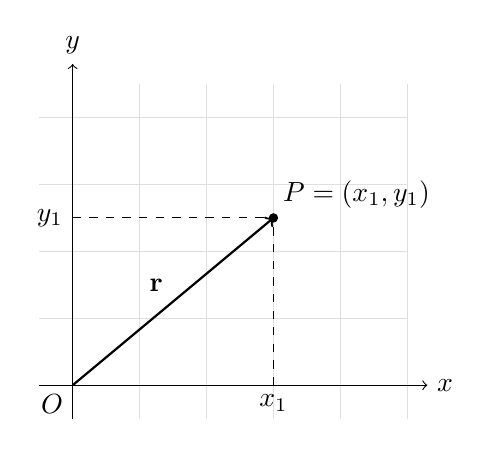
\begin{tikzpicture}[scale=0.85]
    \draw[step=1, gray!25, very thin] (-0.5,-0.5) grid (5.0,4.5);
    \draw[->] (-0.5,0) -- (5.3,0) node[right] {$x$};
    \draw[->] (0,-0.5) -- (0,4.8) node[above] {$y$};
    \draw[dashed] (3,0) -- (3,2.5);
    \draw[dashed] (0,2.5) -- (3,2.5);
    \draw[->, thick] (0,0) -- (3,2.5) node[midway, above left] {$\mathbf{r}$};
    \fill (3,2.5) circle (2pt);
    \node[above right] at (3,2.5) {$P=(x_1,y_1)$};
    \node[below] at (3,0) {$x_1$};
    \node[left] at (0,2.5) {$y_1$};
    \node[below left] at (0,0) {$O$};
\end{tikzpicture}
\end{center}

The position vector depends on the coordinate system. If we choose a different origin or different axes, the coordinates of the same physical point may change. This is not a contradiction. Coordinates are not the point itself. Coordinates are a numerical description of the point after a coordinate system has been chosen.

\subsection{Motion as changing position}

A body is in motion when its position changes in time. This means that the coordinates of the point are functions of time.

In one dimension we write

\[
x = x(t).
\]

In two dimensions we write

\[
x = x(t), \qquad y = y(t),
\]
or, in vector form,

\[
\mathbf{r}(t) = (x(t),y(t)).
\]

In three dimensions we write

\[
\mathbf{r}(t) = (x(t),y(t),z(t)).
\]

This notation is important. The symbol \(t\) represents time. The expression \(\mathbf{r}(t)\) means that position depends on time. If we choose a particular value of time, we obtain the position of the body at that time.

For example, if

\[
\mathbf{r}(t) = (t,t^2),
\]

then at \(t=0\),

\[
\mathbf{r}(0) = (0,0).
\]

At \(t=1\),

\[
\mathbf{r}(1) = (1,1).
\]

At \(t=2\),

\[
\mathbf{r}(2) = (2,4).
\]

Thus one formula describes many positions. It tells us where the point is at each time.

\begin{center}
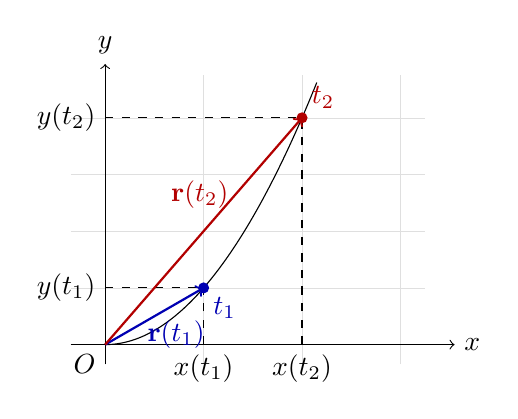
\begin{tikzpicture}[x=1.25cm,y=0.72cm]
    \draw[step=1, gray!25, very thin] (-0.35,-0.35) grid (3.25,4.75);
    \draw[->] (-0.35,0) -- (3.55,0) node[right] {$x$};
    \draw[->] (0,-0.35) -- (0,4.95) node[above] {$y$};
    \draw[domain=0:2.15, smooth, samples=90] plot (\x,{\x*\x});

    \draw[dashed] (1,0) -- (1,1);
    \draw[dashed] (0,1) -- (1,1);
    \draw[dashed] (2,0) -- (2,4);
    \draw[dashed] (0,4) -- (2,4);

    \draw[->, thick, blue!70!black] (0,0) -- (1,1);
    \draw[->, thick, red!70!black] (0,0) -- (2,4);

    \fill[blue!70!black] (1,1) circle (2pt);
    \fill[red!70!black] (2,4) circle (2pt);

    \node[blue!70!black, below right] at (1,1) {$t_1$};
    \node[red!70!black, above right] at (2,4) {$t_2$};
    \node[blue!70!black] at (0.72,0.18) {$\mathbf{r}(t_1)$};
    \node[red!70!black, left] at (1.35,2.65) {$\mathbf{r}(t_2)$};

    \node[below] at (1,0) {$x(t_1)$};
    \node[below] at (2,0) {$x(t_2)$};
    \node[left] at (0,1) {$y(t_1)$};
    \node[left] at (0,4) {$y(t_2)$};
    \node[below left] at (0,0) {$O$};
\end{tikzpicture}
\end{center}

The curve shows the possible positions of the point. The labels \(t_1\) and \(t_2\) mark two different moments of time. At each moment, the point has a different position vector. The vector itself is not the object that moves; it is the mathematical description of the position of the moving point at that time.

\subsection{Trajectory}

The set of all positions occupied by a moving point is called its trajectory. The trajectory is the curve traced by the moving point in space.

It is important to distinguish between the motion and the trajectory. The trajectory is the geometric curve. The motion contains more information, because it tells us where the point is at each moment of time.

Two different motions may have the same trajectory. For example,

\[
\mathbf{r}_1(t) = (\cos t,\sin t)
\]
and
\[
\mathbf{r}_2(t) = (\cos 2t,\sin 2t)
\]

both describe points moving on the unit circle, because in both cases

\[
x^2+y^2 = 1.
\]

However, these two motions are not identical. The second parametrization goes around the same circle differently as time changes. The path is the same, but the time description is different.

This is one reason why parametric descriptions are so important in physics. Geometry alone tells us the shape of the path. Kinematics needs more: it needs the position as a function of time.

\subsection{Motion along a straight line}

The simplest example is motion along a straight line. In one dimension we may write

\[
x(t) = x_0 + at,
\]

where \(x_0\) and \(a\) are constants. At this stage \(a\) is only a parameter in the formula. We will interpret such parameters more deeply after introducing velocity.

If \(x_0=1\) and \(a=2\), then

\[
x(t) = 1+2t.
\]

At \(t=0\),

\[
x(0)=1.
\]

At \(t=1\),

\[
x(1)=3.
\]

At \(t=2\),

\[
x(2)=5.
\]

The position changes along one axis. The trajectory is a line. The formula tells us not only the line on which the point lies, but also the position of the point at every time.

In two dimensions, a straight-line motion can be written as

\[
\mathbf{r}(t) = \mathbf{r}_0 + t\mathbf{a},
\]
where

\[
\mathbf{r}_0 = (x_0,y_0)
\]
and

\[
\mathbf{a} = (a_x,a_y).
\]

In coordinates this means

\[
x(t)=x_0+a_xt,
\]
\[
y(t)=y_0+a_yt.
\]

As \(t\) changes, the point moves along a straight line in the plane.

\subsection{Motion along a parabola}

Consider the position

\[
\mathbf{r}(t) = (t,t^2).
\]

This means

\[
x(t)=t,
\]
and

\[
y(t)=t^2.
\]

If we eliminate the parameter \(t\), we get

\[
t=x,
\]
and therefore

\[
y=x^2.
\]

So the trajectory is a parabola.

The parametric description

\[
\mathbf{r}(t)=(t,t^2)
\]

contains time information. The equation

\[
y=x^2
\]

contains only the shape of the trajectory. It tells us which curve is traced, but not how the point moves along the curve as time passes.

Another parametrization may give the same parabola with a different time description. For example,

\[
\mathbf{r}(t) = (2t,4t^2)
\]

also satisfies

\[
y=x^2,
\]

because if \(x=2t\), then \(t=x/2\), and

\[
y=4t^2=4\left(\frac{x}{2}\right)^2=x^2.
\]

The same geometric curve can therefore be produced by different time parametrizations.

\subsection{Motion along a circle}

Now consider

\[
\mathbf{r}(t)=(R\cos t,R\sin t),
\]

where \(R>0\) is a constant.

Then

\[
x(t)=R\cos t,
\]
and

\[
y(t)=R\sin t.
\]

We can check what geometric curve this describes. We compute

\[
x^2(t)+y^2(t)
=
R^2\cos^2 t+R^2\sin^2 t.
\]

Using

\[
\cos^2 t+\sin^2 t=1,
\]

we obtain

\[
x^2(t)+y^2(t)=R^2.
\]

Thus the point moves along a circle of radius \(R\) centered at the origin.

Again, the equation

\[
x^2+y^2=R^2
\]

describes the circle as a geometric object. The parametric formula

\[
\mathbf{r}(t)=(R\cos t,R\sin t)
\]

describes the position on the circle at each time.

We may also write

\[
\mathbf{r}(t)=(R\cos(\omega t),R\sin(\omega t)),
\]

where \(\omega\) is a constant. This describes the same circle, but the time dependence is different. The parameter \(\omega\) controls how rapidly the argument of the trigonometric functions changes. We will return to the meaning of this when we discuss velocity and circular motion.

\subsection{What position tells us and what it does not tell us}

A function \(\mathbf{r}(t)\) is the complete kinematic description of position. It tells us where the point is at every time. From it, we can find the trajectory by looking at the set of all points \(\mathbf{r}(t)\).

However, position alone is not the end of the description. Once we know how position depends on time, we naturally ask how fast the position changes and in what direction it changes. This question leads to velocity.

Before moving on, the reader should remember the following points:

\begin{itemize}
    \item Motion is described by position as a function of time.
    \item In one dimension, position is written as \(x(t)\).
    \item In two or three dimensions, position is written as a vector \(\mathbf{r}(t)\).
    \item The trajectory is the curve traced by the moving point.
    \item The trajectory is not the same as the full motion.
    \item Different time parametrizations may describe the same geometric curve.
    \item In physics, the time dependence is essential.
\end{itemize}
